%!TEX root = ../thesis.tex
%*******************************************************************************
%*********************************** Eight Chapter *****************************
%*******************************************************************************

\chapter{Data quantified from iPG (blood flow), Doppler ultrasound, LDF and PPG}  %Title of the First Chapter
\label{chapter data collection}

\ifpdf
\graphicspath{{Chapter8/Figs/Raster/}{Chapter8/Figs/PDF/}{Chapter8/Figs/}}
\else
\graphicspath{{Chapter8/Figs/Vector/}{Chapter8/Figs/}}
\fi

The entire experiment was also inclusive of the measurement of physiological changes caused using another set of instruments. As mentioned in chapter \ref{chapter procedure}, devices such as an Electrocardiogram, Doppler Ultrasound, Laser Doppler Flowmetry and PPG in the red spectrum were used to collect data pertaining to the changes in flow and volume across different sections of the forearm and fingers. 

The ECG was used to record the heart's electrical signals and its synchronicity with other signals. The time difference between the ECG's R-wave and the systolic peak of other signals produces what is known as the pulse transit time (PTT), which is useful in determining other physiological parameters including blood pressure~\cite{liu2017cuffless}. The Doppler ultrasound, which was situated close to the radial artery on the wrist, was used to estimate the pace of blood flow at this point. The PPG placed on the index finger provides crucial information about the changes of volume in the vascular bed close to the fingers' area. Finally, the Laser Doppler Flowmetry attached to the mid-section of the forearm is used to gauge the changes of RBC in the vascular bed around the arm. 

\section{Measurements from the ECG device}
\label{section comparison 1}
The ECG signals provided information concerning the electrical activity of the heart during the study. Therefore, extreme changes occurring in the heart rate or shape could not be registered through the test unless there was a bad connection. The data that was gathered also served as a clock reference during the data processing. Figure \ref{fig:ECG} illustrates the typical ECG for one of the participants.

\begin{figure}[!htbp]
	\centering
	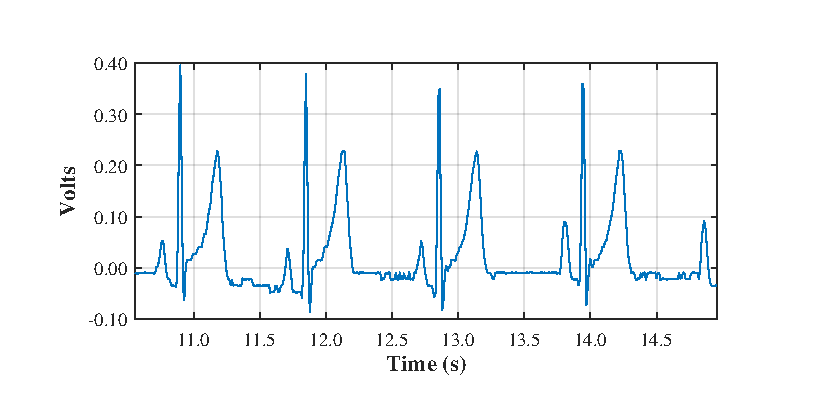
\includegraphics{figure19}    
	\caption[ECG measurement acquired by the system]{ECG measurement from one of the participants. The points can be clearly identified as P, Q, R, S and T as presented in the figure \ref{fig:heart cycle}. This signal did not change during the entire experiment.}
	\label{fig:ECG}
\end{figure} 

All the detected waveforms were typical and provided sufficient information about the characteristic peaks in an ECG waveform. The points P, Q, R, S and T were visible in all the signals. Nonetheless, participant 1 showed an elevated T-wave, which is presumably attributed to his athletic vocation. He said that he had a ventricular hypertrophy, which implies that one of his ventricles got enlarged.  

\section{Blood flow calculation from arterial pulses signal}
\label{section apa flow arterial pulses}
Thus far, blood flow has been analysed from occlusive methods that incorporated the techniques described in section \ref{section literature VOP}. However, these procedures necessitate mechanical occlusion to produce an increase in volume within the forearm that is being measured. Nevertheless, this can oftentimes be uncomfortable, particularly when the pressure is applied above the systolic value or when the person is unable to tolerate restricted blood flow.

For such cases, analysing the waveform offers key information about various aspects of blood flow. The rush of blood into the vessel leads to a tiny surge in volume within the limit of potential electrodes, which then can be translated into a quantifiable blood flow. It is imperative to have a device that is sensitive enough to detect these changes in order to provide an accurate estimation of the blood flow (speed). As mentioned in section \ref{section iPG waveforms}, the waveform contained within the basal impedance got amplified by the device, thereby attaining a great level of detail.

In fact, different studies have demonstrated that it is indeed possible to calculate blood flow by analysing the APA waveform \cite{costeloe1980continuous, yamakoshi1980limb, porter1985measurement, corciova2011peripheral, brown1975impedance, marks1985computer}. Here, the change of impedance used to perform this calculation takes place between the foot of the wave and the systolic peak. This $\Delta Z$ is used to calculate blood flow by applying Nyboer's equation \ref{eq:nyober dV}.

\begin{figure}[!htbp]
	\centering
	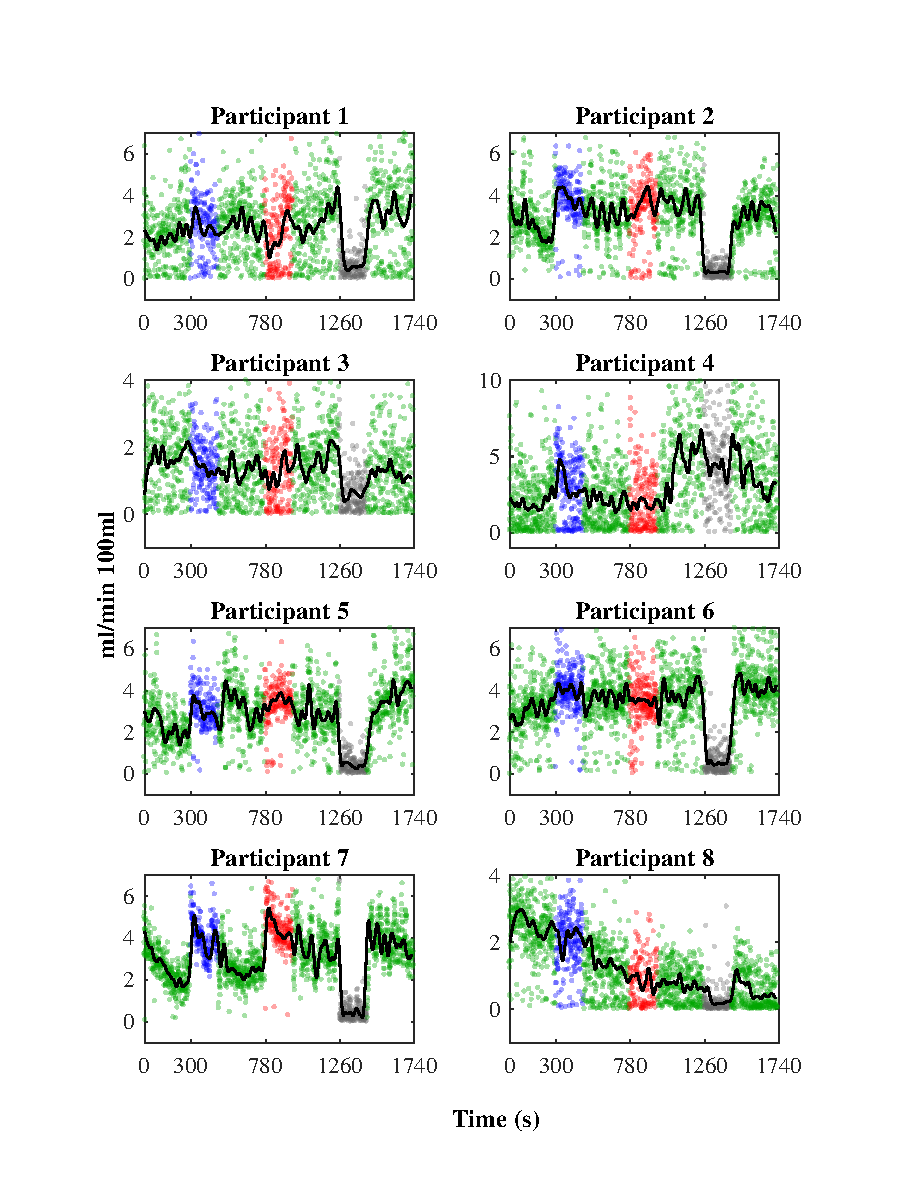
\includegraphics[width=0.85\textwidth,trim={1.5cm 0.5cm 1.5cm 1.5cm},clip]{figure_apa_8}
	\caption[Blood flow calculated from the impedance plethysmography waveform at the time of the whole expetiment]{Blood flow calculated from the impedance plethysmography for all the participants during the whole experiment. Each dot signifies the peak value of the waveform that has been converted into flow (\si{\bfv}). The green dotted area denotes the baselines measurements (regions 1,3,5 and 7). The region 2 (venous occlusion) is represented by the blue dots; arterial occlusions (region 4) are in red and total occlusions (region 6) are in grey.}
	\label{fig:blood_flow_plethysmography}
\end{figure}

Figure \ref{fig:blood_flow_plethysmography} illustrated the flow of blood derived from the amplitude of systolic peak throughout the entire experimental session. Green dots indicate blood flow measurements taken during baseline readings (regions 1, 3, 5 and 6). Meanwhile venous occlusion is shown in blue, partial arterial occlusion in red, and total obstruction in grey. The dark line drawn above the signals corresponds to the smoothing of each measurement event using \textit{robust loess} method of the \textit{smooth} command in Matlab. Overseeing the amplitude transition in every region will help explain how the flow changes with each occlusive event. The value of the calculated blood flow depicted in the figure excludes the negative sign that denotes the direction of flow relative to the potential electrodes.

As portrayed in this figure, between each transition - in the middle of baseline and occlusion - some participants clearly described the marked shifts in the calculated flow. In most participants, when the venous occlusion occurred, the changes between baseline and venous occlusion created a blood surge that was followed by a tendency for the flow to stabilise. Notably, the increment of blood flow in participant 2 occurred prior to the venous occlusion because the obstruction probably commenced before \SI{300}{\second} and the pressure exerted on the arm was rather slow. Meanwhile there are other instances where the flow change took place at such a quick pace that an entirely blank space can be seen to connect both events, as was seen in participants 5 and 7. This scenario, in contrast to participant 2, was more probable since the cuff was inflated at a faster pace, which led to a sudden change in flow, as opposed to a gradual one. However, it could also be correlated with a physiological bodily response such as vasodilation response, where one reacts faster than others. Finally, participant 8 was an exception to this rule and experienced a decline in the calculated flow, which was followed by a period of stabilisation. A flow surge was not identifiable in this participant.

Between venous occlusion and the return to baseline in region 3, the cuff was swiftly deflated so as to restore blood flow to the normal level. However, the calculated data suggests that no extreme changes were observed in the blood flow between these two sections immediately after the release of blockage. As noted before, most participants, except partakers 5 and 7, did not experience significant changes between these two sections, indicating a slight change in blood flow. This can be attributed to a hyperaemic effect where as soon as the pressure is released off the cuff, the blood in the vessels of the forearm rushes out to the upper part of the arm. Subsequently, the blood flow tended to stabilise towards an average value.

Similarly, as seen between regions 1 and 2, the change between baseline (region 3) and partial arterial occlusion (region 4 - red colour) generated alterations in the calculated blood flow. Some participants, such as partakers 6 and 7, experienced a rapid surge in blood flow after the occlusion followed by a settlement in the blood velocity, where the latter becomes more prominent. Meanwhile others such as participants 1, 2, 3 and 5 showed a Gaussian bell-shaped flow during the occlusion. Evidently, their flow did not set in a mean value. The only ones that enacted a different behaviour were participants 4 and 8, who did not experience a significant change. However, the continuous change of amplitude in participant 8 became prominent at this point, which is in contrast to the remaining participants.

The change occurring between partial arterial occlusion (red dotted section) and baseline entailed a similar effect as the one described for releasing the pressure of venous blockage. Most participants had a decreased blood flow, immediately upon the release of cuff's pressure, possibly due to a hyperaemic effect. At this point, participant 4 began exhibiting random blood flow readings.

Total occlusion (grey dots) evinced an expected response in nearly all the members. When the blood flow was completely stopped, its calculated value was expected to be zero. In this case, the device could successfully detect these changes. Participant 4 was the lone exception who again displayed random results. There were strong indications that there could be something wrong with his measurements. Upon the release of tourniquet, the blood flow returned in an exponential form and was then set to an average value. In this case, the hyperaemic effect became more visible. Importantly, participant 8 witnessed a decline in blood flow towards the midpoint of the test. This event concurs with the partaker's expression of not feeling too well by the end of the test. It can be speculated as pure coincidence, or it could be that the device was indeed able to detect these physiological changes within him.

It is likely that there is a blood surge when an occlusion occurs from the impedance computation. Thereafter, the blood flow tends to stabilise at an average value. After the release of blockage, it seems that in certain cases, the flow tends to decrease; in other instances, no apparent change is found. The following sections will extrapolate on the findings of the change in median blood flow during each occlusive event.

\subsection{Blood flow change during venous occlusion}
\label{sectio results 3.1}
The following are the results of calculating the median blood flow between the baseline in region 1, venous occlusion in region 2, and the return baseline after the release of cuff's pressure in region 3. To reiterate, the results do not signify an absolute value, dropping the negative sign as this is indicative of the direction of the flow relative to the electrodes. Table \ref{tbl:blood_flow_iPG_venous} sums up the results obtained by the measurement flow in the scale \si{\bfv}. The mean blood flow in region 1 was about \SI{2.283(0437)}{\bfv}. When the venous occlusion occurred by inflating the cuff below the diastolic value, the average blood flow calculated in region 2 stood at \SI{3.034(0938)}{\bfv}. It can be clearly seen that there was an increase of blood flow in approximately \SI{33}{\percent} during this portion of the experiment. This increment in blood flow could be attributed to a physiological response. It appears as if a vasodilation process allowed for the retention of extra blood in the venous circulation. However, study members 3 and 8 showed a decrease in blood flow during this transition of nearly \SI{0.386(0011)}{\bfv}. The latter does not come as a surprise, as it was noted before, that all his recordings started to go downwards from the commencement of the test. In the case of participant 3, the obtained data did not appear to be distributed towards the mean. Therefore, it is possible that there are a significant number of outliers within its measurement, which makes it difficult to extract the actual median blood flow. 

Clearly, there is a decrease in blood flow when the cuff's tension was released so as to return to the baseline signal.  Six out of eight of the participants witnessed a reduced flow rate during this section of the experiment. The average blood flow for region 3 stood at nearly \SI{2.409(0885)}{\bfv}, equivalent to a \SI{5.5}{\percent} difference with the initial baseline at region 1. On the other hand, participants 1 and 5 did not witness this reduction, but only a slight increase of below \SI{0.09}{\bfv} or \SI{3.9}{\percent} increment as compared to the original reference signal.

\begin{table}[h]
	\caption[Mean blood flow during venous occlusion]{Mean blood flow calculated form the plethysmography wave for baseline (region 1), venous occlusion (region 2) and return to baseline (region 3)}
	\label{tbl:blood_flow_iPG_venous}
	\centering
	\begin{tabular}{l
			*{3}{S[table-format=1.3]@{\,\( \pm \)\,}S[table-format=1.3]} %Format for Z+-std
		}
		\toprule
		& \multicolumn{2}{c}{\textbf{Region 1}}
		& \multicolumn{2}{c}{\textbf{Region 2}}
		& \multicolumn{2}{c}{\textbf{Region 3}}  \\
		& \multicolumn{2}{c}{\small{\si{[\bfv]}}}
		& \multicolumn{2}{c}{\small{\si{[\bfv]}}}
		& \multicolumn{2}{c}{\small{\si{[\bfv]}}} \\\midrule
		Participant 1 & 2.046  & 1.772 & 2.688  & 1.638 & 2.710  & 1.481 \\
		Participant 2 & 2.516  & 1.185 & 3.766  & 1.161 & 3.119  & 1.252 \\
		Participant 3 & 1.794  & 1.282 & 1.416  & 0.796 & 1.325  & 1.260 \\
		Participant 4 & 1.811  & 2.032 & 3.296  & 2.010 & 1.748  & 1.959 \\
		Participant 5 & 2.033  & 1.082 & 3.024  & 0.947 & 3.110  & 1.277 \\
		Participant 6 & 3.054  & 1.289 & 4.019  & 1.146 & 3.566  & 1.330 \\
		Participant 7 & 2.555  & 0.930 & 3.993  & 0.924 & 2.483  & 0.827 \\
		Participant 8 & 2.461  & 0.874 & 2.068  & 0.901 & 1.207  & 0.729 \\
		\bottomrule
	\end{tabular}
\end{table}

\subsection{Blood flow change during partial arterial occlusion}
\label{section apa 3.2}
The change of blood flow between the baseline (region 3) and partial arterial occlusion (region 4) was not as apparent as the response observed in the previous section, where most participants showed a surge in their calculated flow rate. It is clear that three out of eight participants did show an increase in their blood flow, whereas the others witnessed a decline.  In general, the average flow rate during the baseline was \SI{2.408(0885)}{\bfv}. Subsequently, during the partial arterial occlusion, the mean blood flow increased in only \SI{8.4}{\percent} to approximately \SI{2.612(1266)}{\bfv}. 

Clearly, this increase was not as prominent as the one that was observed all along the venous occlusion. Indeed, participants 2, 5 and 7 exhibited an increment in their blood flow with a centre of \SI{0.889(0925)}{\bfv}; in particular, the latter witnessed the greatest change in blood flow. Conversely, the remaining participants observed a small drop in their blood flow, with an average of \SI{-0.208(0180)}{\bfv}.

When the upper arm pressure was released in region 5, most of the participants were expected to experience a decline in their flow rate. However, this was not the case. At this stage, the average blood flow stood at \SI{2.973(1293)}{\bfv}, equivalent to an increment of \SI{23}{\percent} from the baseline region 3. Three study members recorded a drop in their rate (5, 7 and 8) with an average of \SI{-0.618(0431)}{\bfv}. The remaining members meanwhile showed a surge in their data of nearly \SI{0.948(1263)}{\bfv}. As previously described in this region, participant 4 exhibited random values entirely outlying the median that was obtained. At this stage, it is not possible to draw a clear conclusion as to whether  an arterial occlusion would indeed result in a increase or decrease of blood flow from the impedance measurement.

\begin{table}[!htpb]
	\caption[Mean blood flow during partial arterial occlusion]{Mean blood flow calculated form the plethysmography wave for baseline (region 3), partial arterial occlusion (region 4) and return to baseline (region5)}
	\label{tbl:blood_flow_iPG_arterial}
	\centering
	\begin{tabular}{l
			*{3}{S[table-format=1.3]@{\,\( \pm \)\,}S[table-format=1.3]} %Format for Z+-std
		}
		\toprule
		& \multicolumn{2}{c}{\textbf{Region 3}}
		& \multicolumn{2}{c}{\textbf{Region 4}}
		& \multicolumn{2}{c}{\textbf{Region 5}}  \\
		& \multicolumn{2}{c}{\small{\si{[\bfv]}}}
		& \multicolumn{2}{c}{\small{\si{[\bfv]}}}
		& \multicolumn{2}{c}{\small{\si{[\bfv]}}} \\\midrule
		Participant 1 & 2.710  & 1.481 & 2.251  & 1.689 & 2.977  & 1.791 \\
		Participant 2 & 3.119  & 1.252 & 3.486  & 1.399 & 3.537  & 1.492 \\
		Participant 3 & 1.325  & 1.260 & 1.299  & 1.025 & 1.647  & 1.132 \\
		Participant 4 & 1.748  & 1.959 & 1.665  & 1.895 & 4.832  & 7.032 \\
		Participant 5 & 3.110  & 1.277 & 3.454  & 0.994 & 2.841  & 1.225 \\
		Participant 6 & 3.566  & 1.330 & 3.417  & 1.197 & 3.866  & 1.558 \\
		Participant 7 & 2.483  & 0.827 & 4.441  & 1.001 & 3.389  & 1.050 \\
		Participant 8 & 1.207  & 0.729 & 0.882  & 0.864 & 0.693  & 0.537 \\
		\bottomrule
	\end{tabular}
\end{table}

\subsection{Blood flow change during total occlusion}
\label{section apa 3.3}
As mentioned in section \ref{section apa 2.3}, during the total occlusion, the APA amplitude was merely a fraction of the baseline waveform.  Therefore, the $\Delta Z$ obtained to calculate the blood flow is a small number, which results in a low or null calculation. In this aspect of the analysis, most of the study members showed a decline in blood circulation rate close to zero.  Table \ref{tbl:blood flow iPG total} makes it clear that nearly all participants posted a significant decline in their blood flow calculation when the blockage was implemented in region 6. Yet again, participant 4 showed a unique response during the occlusion as the median blood flow did not get close to zero. Beyond all, the median calculated blood flow during the baseline region 5 was nearly \SI{2.972(1210)}{\bfv}. Meanwhile at the time of the brachial arterial constriction, the flow rate lowered to nearly \SI{0.3953(1412)}{\bfv}. Normally, one would expect the reading to show zero as no blood flow passed through the forearm. However, this could be due to an error of equipment measurement induced by noise which was picked up by the device. 

After the withdrawal of tourniquet, the blood flow recovered exponentially, portraying a fast return to the baseline accompanied by an overshot peak and followed by the settlement towards a midpoint, as indicated by figure \ref{fig:blood_flow_plethysmography}. This shape is typical of a hyperaemia where the return of blood flow produces such an overshot response, owing to the rapid filling of the vessels. The mean blood flow in region 7 stood at about \SI{2.892(1332)}{\bfv}, which is very close to the original baseline region 5. As a matter of fact, the reduction in calculated flow was around \SI{2.6}{\percent}. Participant 8 had an anticipated decline in the flow rate prior to the blockage and before signalling a spike. This is fascinating because these changes occurred in a blood flow of below \SI{1}{\bfv}; yet, this device was able to notice the swing of blood flow rate. At this stage, the sensitivity for the calculation of small changes in blood flow requires improvement because it detected flow values in other participants when there was an absence of plethysmography signal. However, it is quite remarkable that the instrument is indeed capable of detecting changes in the trend.

\begin{table}[!htbp]
	\caption[Mean blood flow during total occlusion]{Mean blood flow calculated form the plethysmography wave for baseline (region 5), total occlusion (region 6) and return to normality (region 7)}
	\label{tbl:blood flow iPG total}
	\centering
	\begin{tabular}{l
			*{3}{S[table-format=1.3]@{\,\( \pm \)\,}S[table-format=1.3]} %Format for Z+-std
		}
		\toprule
		& \multicolumn{2}{c}{\textbf{Region 5}}
		& \multicolumn{2}{c}{\textbf{Region 6}}
		& \multicolumn{2}{c}{\textbf{Region 7}}  \\
		& \multicolumn{2}{c}{\small{\si{[\bfv]}}}
		& \multicolumn{2}{c}{\small{\si{[\bfv]}}}
		& \multicolumn{2}{c}{\small{\si{[\bfv]}}} \\\midrule
		Participant 1 & 2.977  & 1.791 & 0.564  & 1.283 & 3.466  & 2.553 \\
		Participant 2 & 3.537  & 1.492 & 0.284  & 0.698 & 2.922  & 1.179 \\
		Participant 3 & 1.647  & 1.132 & 0.567  & 0.751 & 1.277  & 1.210 \\
		Participant 4 & 4.832  & 7.032 & 4.350  & 2.868 & 3.786  & 4.128 \\
		Participant 5 & 2.841  & 1.225 & 0.342  & 0.687 & 3.500  & 1.645 \\
		Participant 6 & 3.866  & 1.558 & 0.448  & 1.190 & 4.103  & 1.489 \\
		Participant 7 & 3.389  & 1.050 & 0.343  & 1.121 & 3.689  & 0.958 \\
		Participant 8 & 0.693  & 0.537 & 0.098  & 0.449 & 0.399  & 0.567 \\
		
		\bottomrule
	\end{tabular}
\end{table}

\section{Blood flow estimation from Doppler ultrasound instrument}
\label{section comparison 2}
As part of the procedure, a Doppler ultrasound was used to estimate blood flow using the radial artery in the wrist as a reference. The raw data produced by this instrument was in the form of volts, which was subsequently converted into more meaningful data using the equations \ref {eq:doppler} and \ref {eq:flow_l/min} which convert this information into units litres per minute (\si{\litre\per\minute}). As described in these equations, the angle was fixed at \SI{45}{\degree} using a laboratory support and a clamp. The cross-sectional area for calculating the blood flow was the median value of~\cite {ashraf2010size}. The head of this ultrasound device was placed as close to the artery as described in the user manual, using a conductive gel as an interface between the skin and the device.

When taking the last participant measurements, the Doppler ultrasound instrument had an electrical problem. Hence, it was not possible to collect the data from participant 8. The data presented in figure \ref{fig:DU flow} and table \ref{tbl:DU flow} comprise of the results of the first seven participants. 
\begin{figure}[!htb]
	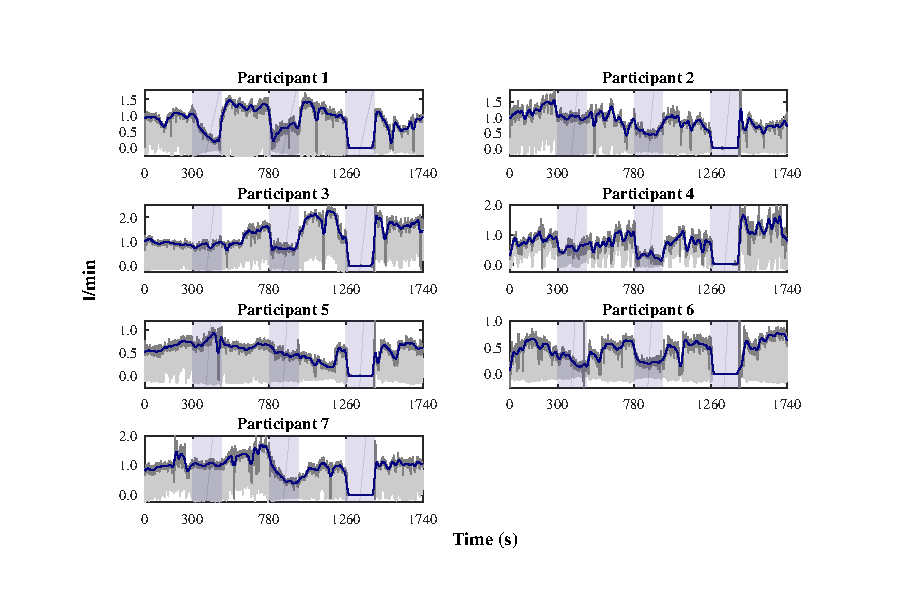
\includegraphics[width=\textwidth,keepaspectratio,trim={1cm 0cm 1.5cm 0cm},clip]{figure_cmp_2}    
	\caption[Blood flow calculated from Doppler Ultrasound device all along the experiment]{Blood flow calculated from the Doppler ultrasound measurements for all the participants during this experiment. The greyed out areas are indicative of the raw sign of the DU waveform whereas the dark blue lines represent the envelope calculated from the peak values. The data was converted into blood flow with units (\si[per-mode=symbol]{\litre\per\minute}).}
	\label{fig:DU flow}
\end{figure}

\subsection{Blood flow estimation from Doppler Ultrasound instrument}
\label{section comparison 2.1}
Figure \ref{fig:DU flow} shows the peak values of the Doppler ultrasound that were converted into the arterial flow rate. The shaded areas signify the occlusive events during the study. The measurements depict the blood flow of the radial artery and the changes occurring during each occlusive event. During venous occlusion, no significant change in arterial flow rate was expected since the brachial artery was not occluded higher than the diastolic pressure. On the other hand, a partial arterial occlusion between the diastolic and systolic pressure curbs the inflow of blood flow towards the radial artery. Finally, at the moment of occluding the brachial artery above the systolic pressure, null blood flow is likely to be displayed.

A qualitative analysis of DU data shows that various participants showed an alteration in their calculated median arterial flow during the venous occlusion in region 2. Whereas others experienced a rapid variation within the first few seconds, others took some time to show a resting point. Participant 1 evidenced an exponential flow rate drop during this aspect of the test. Further, participants 2 and 4 displayed a swift decline within the first few seconds followed by a settling at a mid-point. However, the remaining participants did not show a significant change in flow rate during this transition. Nevertheless, the quantified data showed in \ref{tbl:DU flow} demonstrated that during the transition between baseline regions 1 and 2, five out of seven participants witnessed a reduction in their median blood flow, being Participant 1 the most obvious among them with a drop of \SI{52.41}{\percent} of the blood speed. The other ones who exhibited a slight decline were partakers 2,3,4 and 6 whose their blood flow was about \SI{25.80(1850)}{\percent}. On the other hand, participants 5 and 7 showed a slight surge in their calculated blood flow in \SI{10.16}{\percent} and \SI{6.25}{\percent}, respectively. Upon the release of the cuff's pressure, most participants showed a recovery within the detected blood flow. Only participants 2 and 5 exhibited a minimal decline.

During the partial arterial occlusion, the arterial blood flow changed unmistakably in all the participants. In this case, it is evident that the narrowing of the brachial artery curbed blood flow in the arm's arterial circulation, altering the flow rate speed that was detected by the DU. As shown by the figure, most participants exhibited a swift change of blood flow as soon as the constriction was applied, with the exception of participant 5. Generally speaking, the reduction of blood flow in the radial artery stood at around \SI{48.79(1191)}{\percent}. As soon as the flow was restored, majority of the participants witnessed a surge in their blood flood caused by a rush of blood within the arterial circulation passing through a quick inflow for a few seconds. However, participant 5 showed a different response which might have been caused by the misalignment of the sensor head.  

\begin{table}[!htb]
	\caption[Mean blood flow calculated from the Doppler Ultrasound]{Mean blood flow calculated form the Doppler Ultrasound waveform during all the regions of the experiment.}
	\label{tbl:DU flow}
	\centering \small
	\begin{tabular}{p{1.9cm}cccccccc}
		\toprule
		& \textbf{Region 1}
		& \textbf{Region 2}
		& \textbf{Region 3}
		& \textbf{Region 4}
		& \textbf{Region 5}
		& \textbf{Region 6}
		& \textbf{Region 7} \\
		& \textbf{[\si[per-mode=symbol]{\litre\per\minute}]}
		& \textbf{[\si[per-mode=symbol]{\litre\per\minute}]}
		& \textbf{[\si[per-mode=symbol]{\litre\per\minute}]}
		& \textbf{[\si[per-mode=symbol]{\litre\per\minute}]}
		& \textbf{[\si[per-mode=symbol]{\litre\per\minute}]}
		& \textbf{[\si[per-mode=symbol]{\litre\per\minute}]}
		& \textbf{[\si[per-mode=symbol]{\litre\per\minute}]} \\\midrule	
		Participant 1 & 0.954 & 0.430 & 1.285 & 0.618 & 1.049 & 0.003 & 0.719 \\
		Participant 2 & 1.211 & 1.014 & 0.967 & 0.546 & 0.843 & 0.002 & 0.712 \\  
		Participant 3 & 0.928 & 0.860 & 1.307 & 0.716 & 1.940 & 0.002 & 1.675 \\  
		Participant 4 & 0.826 & 0.581 & 0.764 & 0.297 & 0.754 & 0.002 & 1.245 \\  
		Participant 5 & 0.643 & 0.708 & 0.655 & 0.483 & 0.348 & 0.003 & 0.606 \\  
		Participant 6 & 0.495 & 0.248 & 0.499 & 0.230 & 0.542 & 0.002 & 0.641 \\  
		Participant 7 & 0.962 & 1.022 & 1.320 & 0.535 & 0.876 & 0.002 & 1.040 \\  	
		\bottomrule
	\end{tabular}
\end{table}

Finally, the tourniquet effect can be noticed in the composition of the signal all along the total occlusion with a sharp decline as soon as the occlusion took place. As expected, no arterial flow was recorded; the minimum values might signify the artefacts in the signals. After releasing the tourniquet, all participants experienced a surge in their flow rate to values of normality. 

\section{Measurements from Laser Doppler Flowmetry}
\label{section comparison LDF}
The LDF device provided raw data in Volts which was subsequently converted into BPU units. This conversion was made possible by applying equation \ref{eq:BPU} to the collected data. As explained in section \ref{section:ldf}, it resulted in an arbitrary unit, which denotes the movement of blood cell beneath the skin's micro-circulatory bed. This unit called BPU refers to the product of the mean number of moving blood cells into the small volume under the probe and the average velocity of moving red blood cells in the forearm. Converting the raw data to BPU unit could be done using the equation \ref{eq:BPU}.

Figure \ref{fig:LDF flow} shows the peaks of the LDF waveform signal in BPU. The grey points are the measurements' raw data. The purple line in this figure represents the smoothed signal averaged per heartbeat. The boxed areas describe the data portions where these occlusions occurred. This plot shows that evidently, the movement of blood cells is affected when an occlusion occurs. Indeed, there is a diminution of the magnitude of signal during each flow restriction. During the course of experiment, the LDF signal was very susceptible to noises; this explains the rationale behind massive peaks witnessed during some of the measurements. In particular, participants 1 and 3 showed a significant number of high peaks. From the qualitative viewpoint, the strong impact on some parts of the data is evident, such as in participants 1 and 4.

\begin{figure}[!htb]
	\centering
	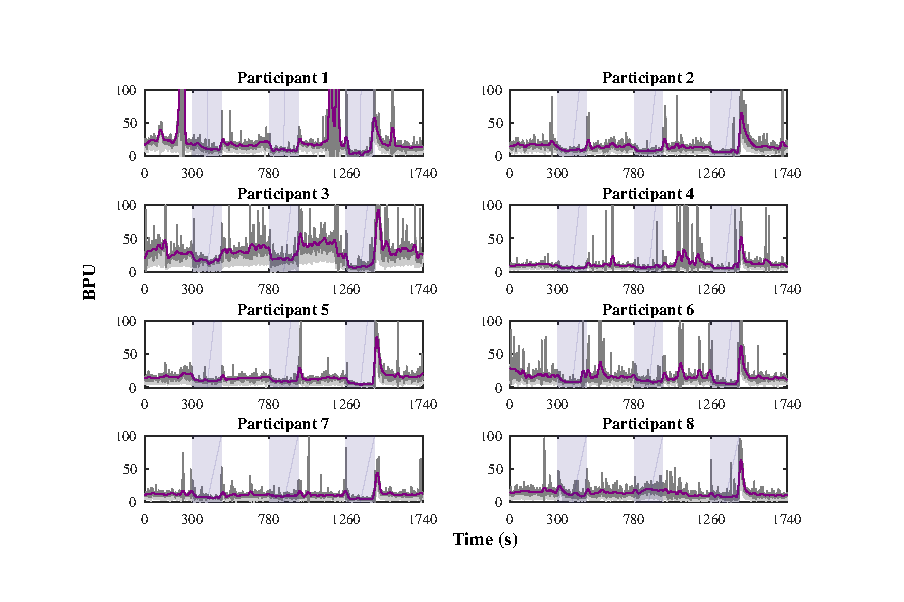
\includegraphics[width=\textwidth,keepaspectratio,trim={1cm 0cm 1.5cm 0cm},clip]{figure_cmp_3}    
	\caption[Results of the LDF in BPU]{Results of the Laser Doppler Flowmetry measurement for all the participants after being converted to BPU. The values presented in purple are equivalent to envelope signal of the peak points.}
	\label{fig:LDF flow}
\end{figure}

Nevertheless, a trend is noticeable in all the participants. During the occlusions, a drop in the red blood cell movement was noticed. It seems that the blockage of venous return in regions 3 and 5 slowed down the movement of RBC in the capillaries. Additionally, during total occlusion, the amplitude reaches its lower values. After the restoration of blood flow, the RBC movement depicted a Gaussian bell shape peak throughout most participants. This hyperaemic effect shows an acceleration of blood cells following the blockage event. While this acceleration is evident in every occlusion, it varies in magnitude with each occlusion. The BPU magnitude is clearly larger on in all participants following the total occlusion. In comparison, two other occlusions created a smaller Gaussian shape as a response where the one that ensued after the partial arterial appears to be slightly bigger. Nevertheless, participant 8 seems to be an exception to this rule. The BPU measurements increased only slightly during the transition from region 3 to 4. Also, in contrast to the other participant's waveforms in the transition from partial arterial occlusion to the baseline in region 5, his mean BPU dropped. The results obtained from this participant could also explain some of the adverse readings that were captured by the iPG signals.

Lastly, during total occlusion, all the mean BPUs of the participants reduced significantly. At a subsequent stage when the tourniquet was released, the rush of blood flow is evident in the hyperaemic effect registered by the instrument, which was also detected by other instruments. Table \ref{tbl:LDF flow} reviews the values of the mean BPU data. These results are in absolute harmony with the figure that was previously analysed.

\begin{table}[!htbp]
	\caption[Calculated media perfusion index from the LDF device in BPU]{Media perfusion index (flux) calculated from the LDF data for all the regions during the experiment.}
	\label{tbl:LDF flow}
	\centering \small
	\begin{tabular}{p{1.9cm}cccccccc}
		\toprule
		& \textbf{Region 1}
		& \textbf{Region 2}
		& \textbf{Region 3}
		& \textbf{Region 4}
		& \textbf{Region 5}
		& \textbf{Region 6}
		& \textbf{Region 7} \\
		& \textbf{[BPU]}
		& \textbf{[BPU]}
		& \textbf{[BPU]}		
		& \textbf{[BPU]}		
		& \textbf{[BPU]}
		& \textbf{[BPU]}
		& \textbf{[BPU]}\\\midrule
		Participant 1 & 23.65 & 11.59 & 17.20 &  9.20 & 19.81 & 5.16 & 14.60 \\  
		Participant 2 & 16.88 &  9.10 & 14.44 &  8.19 & 13.17 & 6.07 & 14.83 \\  
		Participant 3 & 29.46 & 17.43 & 32.86 & 19.76 & 41.80 & 7.83 & 33.87 \\  
		Participant 4 &  9.81 &  6.14 &  9.53 &  6.99 & 14.11 & 5.94 & 12.19 \\  
		Participant 5 & 15.56 & 10.35 & 13.85 &  9.28 & 14.02 & 4.73 & 18.03 \\  
		Participant 6 & 18.66 &  8.80 & 16.03 &  9.56 & 15.06 & 6.60 & 14.56 \\  
		Participant 7 & 11.96 &  7.25 & 10.37 &  9.51 & 10.24 & 5.08 & 11.91 \\  
		Participant 8 & 15.54 & 12.40 & 13.85 & 17.93 & 12.29 & 8.40 & 10.97 \\  
		\bottomrule
	\end{tabular}
\end{table}


\section{Measurements from the PPG Red-light signal}
\label{section comparison PPG}
The photoplethysmographic device provided key information about the change of volume within the vascular bed underneath the skin. It is capable of detecting venous or arterial blood change in accordance to the light wavelength ~\cite{almond1988noninvasive}. The finger probe used throughout the experiment comprised of red and infrared sensors. Nevertheless, the red-light information was collected because it was more sensitive to the changes made in the venous blood. The device employed in this experiment has an output port that provides the unprocessed raw photoplethysmography waveform. Similarly, as is evident in the iPG signal, the PPG comprises of DC and AC components. The DC portion of this signal is equivalent to the blood volume noted under the light beam. Moreover, it contains data about the respiratory rate in addition to other physiological information, which is not necessary for this experimental setting. On the contrary, the magnitude of AC component changes synchronously with the cardiac cycle and blood volume under the capillaries. 

The raw signal displayed in \ref{fig:RED PPG} reveals the DC (left side) and the AC (right side) components of all the participants. Additionally, within the plot, the shaded regions are indicative of each occlusive event during the experiment. The DC component of the signal was obtained by decoding the bottom values that envelope the raw PPG waveform. In other words, these are points on the foot of the waveform.  In addition, the AC component of this signal was obtained by subtracting the low envelope of the raw data. Furthermore, the resultant waveform was inverted to permit only the dynamic element of the signal. Lastly, the peaks detected from the plethysmography waveform were redrawn in black, thus highlighting the peak values during all the occlusive events.

\begin{figure}[!htbp]
	\centering
	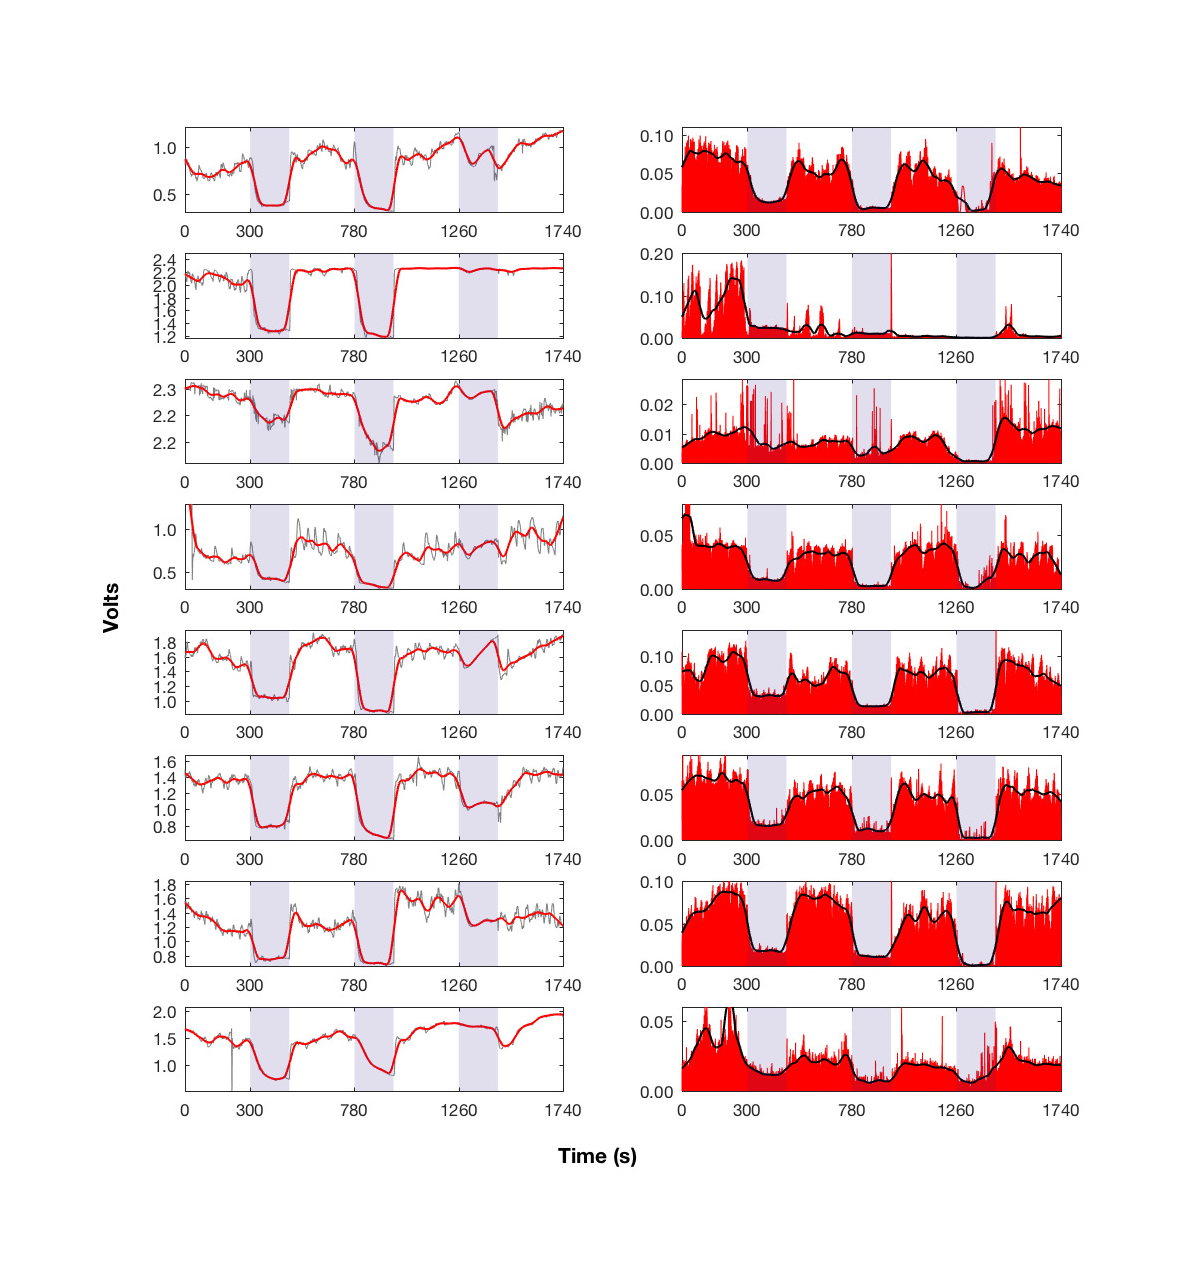
\includegraphics[width=\textwidth,keepaspectratio,trim={1cm 0cm 0cm 0 cm},clip]{figure_cmp_4}
	\centering
	\begin{minipage}[t]{.45\linewidth}
		\centering
		\subcaption{DC component of the PPG waveform for each of the participants}\label{fig:RED PPG AC}
	\end{minipage}%
	\centering
	\begin{minipage}[t]{.45\linewidth}
		\centering
		\subcaption{AC component of the PPG waveform for each of the participants}\label{fig:RED PPG DC}
	\end{minipage}
	\caption[PPG red wavelength measurments, AC and DC components]{PPG measurements using the red spectrum. The plots show the DC and AC components of the waveform. The shaded areas represent the occlusion events during the venous occlusion (region 2), partial arterial occlusion (region 4) and total occlusion (region 6))}
	\label{fig:RED PPG}
\end{figure}

\subsection{Changes in the DC component of the signal}
\label{section comparison 4.1}
After analysing the DC signal, it can be seen from the figure that all participants showed a definite decline in their DC components during venous occlusion (region 2) and partial arterial occlusion (region 4). It illustrates that the DC value reduced dramatically in most participants following the occlusive event. Nevertheless, some participants displayed an exponential drop in their recordings, as shown in participants 3 and 8 during both occlusive events. 

The visible changes of the DC value is confirmed when analysing the mean values of the DC data presented in Table \ref{tbl:PPG RED-DC}. From there on, the calculated average baseline prior to the occlusions were \SI{1.44(055)}{\volt} for Region 1 and \SI{1.51(054)}{\volt} for Region 3.  In contrast, the DC components dropped about \SI{0.435(0210)}{\milli\volt} and \SI{0.528(0247)}{\milli\volt} during the occlusive transitions for region 2 and region 4, respectively. When comparing the DC values between both events, it can be seen that difference between the two is not significant - only \SI{4.47}{\percent}. Nevertheless, during total occlusion, the signals were erratic with no definite shape or direction. Some participants did exhibit a slight decline, but others did not display significant changes. In general, the DC data provided valuable information during the venous and partial arterial occlusion, but no conclusive results could be observed when the blood flow stopped altogether. 

\begin{table}[!htbp]
	\caption[Mean peak value of the PPG DC signal for all participants in all regions]{Mean peak value of the PPG DC signal for all the participants in all the regions.}
	\label{tbl:PPG RED-DC}
	\centering \small
	\begin{tabular}{p{1.9cm}cccccccc}
		\toprule
		& \textbf{Region 1}
		& \textbf{Region 2}
		& \textbf{Region 3}
		& \textbf{Region 4}
		& \textbf{Region 5}
		& \textbf{Region 6}
		& \textbf{Region 7} \\
		& \textbf{[\si{\volt}]}
		& \textbf{[\si{\volt}]}
		& \textbf{[\si{\volt}]}		
		& \textbf{[\si{\volt}]}		
		& \textbf{[\si{\volt}]}
		& \textbf{[\si{\volt}]}
		& \textbf{[\si{\volt}]}\\\midrule
		Participant 1 & 0.75 & 0.44 & 0.91 & 0.43 & 0.94 & 0.91 & 1.03 \\  
		Participant 2 & 2.09 & 1.38 & 2.22 & 1.33 & 2.25 & 2.24 & 2.24 \\  
		Participant 3 & 2.24 & 2.20 & 2.24 & 2.16 & 2.23 & 2.24 & 2.20 \\  
		Participant 4 & 0.76 & 0.46 & 0.80 & 0.36 & 0.72 & 0.79 & 0.89 \\  
		Participant 5 & 1.60 & 1.07 & 1.73 & 0.93 & 1.66 & 1.64 & 1.64 \\  
		Participant 6 & 1.36 & 0.84 & 1.38 & 0.76 & 1.41 & 1.08 & 1.35 \\  
		Participant 7 & 1.26 & 0.79 & 1.25 & 0.75 & 1.56 & 1.32 & 1.34 \\  
		Participant 8 & 1.48 & 0.88 & 1.48 & 1.07 & 1.64 & 1.71 & 1.70 \\  
		\bottomrule
	\end{tabular}
\end{table}

\subsection{Changes in the AC component of the signal}
\label{section comparison 4.2}
The AC component also produced a notable swing of magnitude during each blockage event. When compared to the DC, the AC signal not only changed its amplitude all along the venous and partial arterial occlusion, but also during the total occlusion, where it reached its minimum magnitude which is consistent with the fact that no change of volume is evident at that precise instant. Reviewing the AC signals qualitatively, participants 2, 3 and 5 exhibited low-quality waveforms since amplitudes were quite close to noise levels  (amplitude < \SI{10}{\milli\volt}). Participant 2 registered noisy waveforms during region 1 of the study and small magnitudes for the remainder of this experiment. Participant 3 meanwhile exhibited low signal amplitude and over peaks during the entire test, although the changes through each occlusion continue to be visible.

\begin{table}[!htbp]
	\caption[Mean peak value of the PPG AC signal for all participants in all regions]{Mean peak value of the PPG AC signal for all the participants in all the regions.}
	\label{tbl:PPG RED-AC}
	\centering \small
	\begin{tabular}{p{1.9cm}cccccccc}
		\toprule
		& \textbf{Region 1}
		& \textbf{Region 2}
		& \textbf{Region 3}
		& \textbf{Region 4}
		& \textbf{Region 5}
		& \textbf{Region 6}
		& \textbf{Region 7} \\
		& \textbf{[\si{\milli\volt}]}
		& \textbf{[\si{\milli\volt}]}
		& \textbf{[\si{\milli\volt}]}		
		& \textbf{[\si{\milli\volt}]}		
		& \textbf{[\si{\milli\volt}]}
		& \textbf{[\si{\milli\volt}]}
		& \textbf{[\si{\milli\volt}]}\\\midrule
		Participant 1 & 724.83 & 180.45 & 546.76 &  66.13 & 490.87 & 109.85 & 441.54   \\  
		Participant 2 & 926.02 & 245.24 & 158.34 & 110.32 &  51.30 &   5.97 &  92.58   \\  
		Participant 3 &  94.21 &  69.72 &  68.76 &  37.19 &  71.62 &  10.54 & 122.67   \\  
		Participant 4 & 436.74 &  92.42 & 315.26 &  37.22 & 354.44 &  58.08 & 296.36   \\  
		Participant 5 & 873.38 & 324.60 & 638.53 & 155.21 & 703.81 &  51.36 & 751.62   \\  
		Participant 6 & 658.05 & 188.75 & 501.10 & 112.57 & 480.41 &  38.14 & 517.01   \\  
		Participant 7 & 731.50 & 190.43 & 746.34 & 125.76 & 547.89 &  26.92 & 660.43   \\  
		Participant 8 & 360.69 & 130.06 & 216.80 &  74.43 & 168.52 &  89.77 & 217.06   \\ 
		\bottomrule
	\end{tabular}
\end{table}

From the numeric point of view, Table \ref{tbl:PPG RED-AC} shows the average values of the amplitude in \si{\milli\volt}. During all baseline measurements (regions 1, 3, 5 and 7), the mean peak value stood at \SI{436.41(11081)}{\milli\volt}. However, it is evident that the overshooting displayed considerably higher values than the mean.  

In general, during venous occlusion, the signal amplitude dropped in all the experiment members in around \SI{422.97(21217)}{\milli\volt}. However, participant 3 was an outlier showing the smallest change (\SI{24.50}{\milli\volt}) in comparison to the remaining signals.  It seems that the poor-quality signal ended up affecting the entire measurement. After the cuff's pressure was released during the transition from venous occlusion to baseline, participants 2 and 3 witnessed a decline in their mean amplitude. Yet again, their poor signal quality caused them to show conclusive measurements. The rest of the partakers recorded a recovery in their peak signal to a peak of nearly \SI{221.28(21124)}{\milli\volt}. 

During partial arterial occlusion in region 4, this device detected the physiological response. In this case, all participants witnessed a drop in their mean PPG signals amplitude of an average of \SI{309.14(21943)}{\milli\volt}. When comparing the mean values during occlusions in region 2 and 4, the signal amplitude in region 4 was slightly lower than the one in region 2 by close to \SI{87.86(4691)}{\milli\volt}, which is the difference between both circulatory occlusions \SI{49.75}{\percent}.

Finally, throughout the total occlusion, all participants exhibited a substantial reduction in their AC amplitudes. This was expected due to the absence of blood flow within the vessels. In entirety, the signals went below \SI{109}{\milli\volt} with an average value of \SI{48.83(3662)}{\milli\volt}. In fact, this confirms that the measurements taken from participants 3 were below this level. 

In conclusion, the PPG waveform witnessed changes of DC and AC components during all the occlusions conducted throughout the study. The DC signal successfully detected changes during both venous and partial arterial occlusions. The difference of their mean DC values during these two events was minimal at only \SI{4.47}{\percent}. Furthermore, during total occlusion, no noticeable change in DC value of the signal was observed.  On the other hand, the AC component effectively distinguished between venous and partial occlusion. The difference between these two regions stood at about \SI{50}{\percent}. Moreover, the signal lost most of its magnitude during total occlusion due to inadequate blood flow.

\section{Conclusion}
\label{section comparison 5}
This chapter described the general changes of the waveforms observed the entire experiment. All the instruments evinced a different response in accordance to the technology used by each one of them. The data obtained from this impedance device was converted into blood flow so as to decipher the changes occurring in venous circulation. The Doppler Ultrasound method recorded changes in the arterial circulation, while the optical techniques exhibited alterations in the microcirculation. 

Converting the impedance APA waveform into blood flow by applying Nyboer equation \ref{eq:nyober dV}, which finds mention in the lecture \cite{costeloe1980continuous, yamakoshi1980limb, porter1985measurement, corciova2011peripheral, brown1975impedance, marks1985computer}, reflected a surge in the blood rate. This increase in the measurement was expected since the flow rate is directly proportional to the amplitude of the impedance. As mentioned in chapter \ref{chapter apa}, the APA waveform depicted an increase of its systolic peak during both venous and partial arterial occlusions. For example, during venous occlusion in region 2, the blood rate increased by nearly \SI{33}{\percent} when compared to the previous baseline in region 1. It appears as if the surge in blood flow might be attributed to a vasodilation response where the cross-sectional area of these veins in the forearm enlarged, which allowed for blood pooling. 

However, comparing venous and partial arterial occlusions produced different results with regard to the rise in blood flow. Although both events witnessed an increase in their waveform systolic peaks, the calculated flow rate during the partial occlusion was \SI{8.4}{\percent} (on average) in region 4. While the blood flow was expected to reduce as the normal artery flow got restricted, the impedimetric measurement presented a slight surge in blood flow. Yet again, it appears that the increase in calculated blood flow might be related to vasodilation caused during the occlusion. The extra blood flowing into the expanded vein may be viewed as a surge in the blood flow rate.

Meanwhile the Doppler Ultrasound method detected changes in the arterial flow. The instrument's sensor was pointing towards the radial artery to provide further information about the changes of arterial inflow within the forearm. However, this approach is ridden with some shortcomings. For example, proper measurements need a person with specific skills to be able to accurately target the vessel under study, such as steady-hand and acute hearing. In addition, it can be difficult for any person to keep a fixed angle of measurements for prolonged periods of time. While some of these issues were addressed during the experiment by using a fix lab clamp, any movement from the participant would end up misaligning the sensor, thus resulting in errors in the recorded data. In general, the instrument detected changes within the arterial flow during both partial arterial and total occlusion. The arterial blood rate reduced to nearly \SI{48.79(1191)}{\percent} during partial arterial occlusion, and practically zero during complete obstruction.

In comparison, the optical methods yielded data about the venous circulation. The PPG in the red spectrum correlated to the venous circulation, whereas the LDF provided details of the blood cells moving into the capillary bed. One of the disadvantages of the optical methods is that the measurement is confined to a small volume, which makes it difficult to accurately ascertain the depth at which the light beam is travelling into the tissue. However, a specialist is not required to take measurements in optical methods, which makes it feasible for an unsupervised operation.



%********************************** %Nomenclature found  *************************************
\nomenclature[z-PTT]{PTT}{Pulse transit time}